\chapter{Black and Scholes model}
\label{BSformula}
\section{Theorem}

Thanks to the work of Black, Scholes and Merton, who received in $1997$ the Nobel price of economy for their contribution (actually Mr. Scholes died in $1995$ then ineligible for the prize), there exists a simple closed form solution to pricing options under a normal model.  

\begin{theoreme}[label = thrm:BSformula]{Black $\&$ Scholes Formula}
If one assumes that the stock price has the following dynamic:

$$S_t = S_0 \exp \{ (r - \frac {\sigma^2} 2) t + \sigma W_t \} $$

where:
\begin{itemize}
\item $(W_t)$ is a brownian motion, 
\item $r \geq 0$ is the risk-free interest rate,  
\item $\sigma > 0$ is the volatility, 
\end{itemize}

then one has the following price for a european call option :

$$ C_{BS}( S_0, K, T, \sigma ) = S_0 \phi ( d_+ ) - e^{-r T } K  \phi( d_- ) $$ 

with : 

$$ d_{\pm} = \frac{1}{\sigma \sqrt{T}  } \left ( \ln(\frac{S_0}{K}) + \left ( r \pm \frac{\sigma^2}{2} \right ) T \right )$$
and $\phi$ being the CDF of a normal distribution.

In the same way, one can price put options : 

$$P_{BS}( S_0, K, T, \sigma ) =  e^{-rT} K \phi(-d_-) - S_0 \phi(-d_+) $$

\end{theoreme}



\begin{remarque}
Under the B$\&$S model, if one assumes the following dynamic for the asset's price:

$$ \frac {dS_t}{S_t} = r dt + \sigma dW_t$$

Then, using Ito's lemma (cf. section \ref{subsection:itoslemma}), one finds that the process follows this dynamic:

$$ S_t = S_0 \exp \left ( (r - \frac 1 2 \sigma^2 )t + \sigma W_t \right ) $$
Then, one recognises a log-normal distribution for $S_t$.

Having a log-normal distribution for our process has a fairly intuitive explaination. An asset can't have a normal distribution even thought its price is generated by a brownian motion for the simple reason that it can grow much higher than it can fall. A price is limited by a lower bound at $0$. Thus, an intuitive way to skew the normal distribution is a log-normal distribution. 

This is also the reason why studying $\ln(S_t)$ is way more common than $S_t$. The former is normally distributed with mean $\tilde{\mu} = \ln(S_0) + (r - \frac 1 2 \sigma^2 )t$ and variance $\tilde{\sigma}^2  = \sigma^2 t$.
\end{remarque}


A few comments on Black and Scholes. Underlying this formula, the authors have put some assumption on the asset:

\begin{itemize}
\item the rate of return on risk free asset is constant,
\item  the risky asset price behaves as a geometric Brownian motion,
\item no dividends.
\end{itemize}

as well as on the market:

\begin{itemize}
\item arbitrage free market,
\item same interest rate for borrowing and lending at the risk free asset,
\item possible to buy and sell any amount of the stock,
\item  no transaction costs.
\end{itemize}

There are some extensions that intend to generalize the theorem, such as Ingersoll in 1976 who included the transaction costs for buying/selling, and Whaley in 1981 who incorporated dividends payouts.

Finally, one can list some limitations to this model:

\begin{itemize}
\item underestimation of extreme moves in the stock, leading to tail risk. It is the financial risk of an asset or portfolio of assets moving more than 3 standard deviations from its current price. One should be cautious with tail risk involving losses which could damage or ruin portfolios, and not the beneficial tail risk of outsized gains
\item assumption of instant, cost less trading, leading to liquidity risk. It is a financial risk that for a certain period of time a given financial instrument cannot be traded quickly enough in the market without impacting the market price.
\item assumption of stationary process, leading to volatility risk. It is the risk of a change of price of a portfolio as a result of changes in the volatility of a risk factor.
\item assumption of continuous time and trading, leading to gap risk. The latter is defined as the risk that a stock's price will fall dramatically from one trade to the next. A gap occurs when a security’s price changes from one level to another (up or down) without any trading in between.
\end{itemize}

\section{Characteristic function of the B$\&$S formula}
\label{anx:charac_BS}



Since a classical result from probability gives that the characteristic function of a normal random variable with mean $\tilde{\mu}$ and variance $\tilde{\sigma}$ is:

$$ \phi(\xi) = \exp \left ( i \xi \tilde{ \mu } - \frac {\tilde{ \sigma }} 2  \xi^2 \right ) $$

Then one deduces the result (\ref{eq:charac_BS}) presented page \pageref{eq:charac_BS}:

$$ \phi_{X_t} (\xi) = \exp \left ( i \xi X_0 + ( r - \frac{ \sigma^2}{2}
) i \xi t - \frac{\sigma ^2 \xi ^2 t}{2} \right ) $$

Using the same idea as presented in \ref{chapteroptionpricing}, we inject the formula above into (\ref{eq:Pis}) and (\ref{eq:super_pricing}). Some examples of pricing for varying strike price are shown in fig. \ref{fig:bsprice1} and in fig. \ref{fig:bsprice2}. The parameters are given in table \ref{table:BSmodels_pricing}.



\begin{table}
\begin{center}
\begin{tabular}{  | m{2.5cm} | m{1.2 cm} | m{1.2 cm}| m{1.2 cm} |  m{1.2 cm} | m{1.2 cm}|  } 
\hline
parameter & $S_0$ &  $V_0$ & $\sigma$ & $r$ & $d$  \\ 
\hline
values &$1$ & $0.1$ & 0.1 & $0$ & $0$  \\
\hline
\end{tabular}
\caption{Set of parameters for pricing with the Black and Scholes model.}
\label{table:BSmodels_pricing}
\end{center}
\end{table}


\begin{figure}
\centering
   \includegraphics[width = 0.75 \textwidth]{../addition_part/images/BS/b&S.png}
   \caption{Price for an option under the B$\&$S Model, exact computation.}
   \label{fig:bsprice1}
\end{figure}


\begin{figure}
\centering
   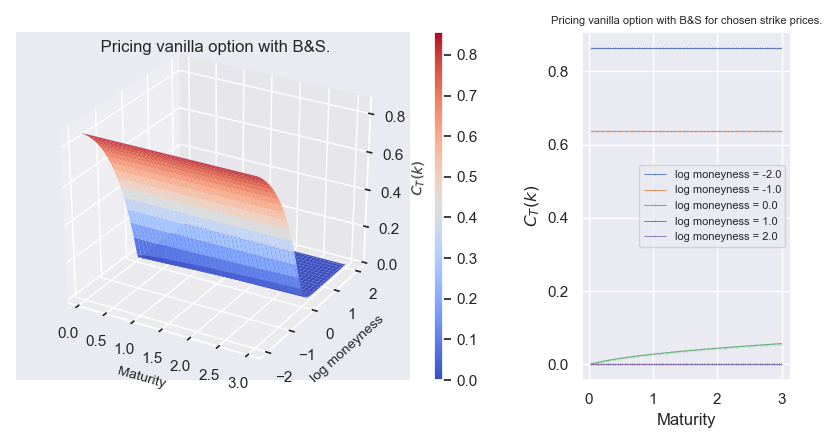
\includegraphics[width = 0.9 \textwidth]{../addition_part/images/BS/b&s_cover.png}
   \caption{Pricing Frontier for an option under the B$\&$S Model, exact computation.}
   \label{fig:bsprice2}
\end{figure}









\section{Inverting B$\&$S formula}
\label{anx:invert_BS}

We are going to prove that equation \ref{eq:IVunique} is unique. In order to do that, we first prove that the function is injective.

A useful fact is 
$$\text{ VEGA } (C_{BS}( S_0, K, T, \sigma )) = \text{ VEGA } (P_{BS}( S_0, K, T, \sigma )) $$ then knowing call's vega gives us put's vega. Notice that the price is not define for $\sigma$ equals to $0$. Thus we derive the derivative on the strictly positive real axis. 


In fact, it can proven that the call price belongs to the class of $C^{\infty}$ functions.


Remember that:
\begin{align*}
C_{BS}( S_0, K, T, \sigma ) &= S_0 \phi ( d_+ ) - e^{-r T } K  \phi( d_- ) 
\end{align*}

and notice:

\begin{align*}
\frac{\partial d_+ }{\partial \sigma }  &= \sqrt T - \frac {d_+} {\sigma} = - \frac {d_-} {\sigma} \\
\frac{\partial d_- }{\partial \sigma }  &= - \frac {d_+} {\sigma} 
\end{align*}

Hence: 

\begin{align*}
\text{ VEGA } (C_{BS}( S_0, K, T, \sigma )) 
&= S_0 \phi' ( d_+ ) \frac{\partial d_+ }{\partial \sigma } 
- e^{-r T } K  \phi'( d_- ) \frac{\partial d_- }{\partial \sigma } \\ 
&= \frac{-S_0}{\sigma \sqrt{2\pi}}{e^\frac{-d_+^2}{2}} d_-
+ \frac{Ke^{-rT}}{\sigma \sqrt{2\pi}}e^{\frac{-d_-^2}{2}} d_+ 
\\
&=\frac{1}{\sqrt{2\pi}}e^{\frac{-d_+^2}{2}}\left[-\frac{S_0 d_-}{\sigma} + \frac{Ke^{-rT}d_+}{\sigma} e^{\frac{d_+^2}{2} - \frac{d_-^2}{2}} \right]\\
&=N'(d_+)\left[-\frac{S_0 d_-}{\sigma} + \frac{Ke^{-rT}d_+}{\sigma} e^{\frac{1}{2}(d_+-d_-)(d_++d_-)} \right]\\
&=N'(d_+)\left[-\frac{S_0 d_-}{\sigma} + \frac{Ke^{-rT}d_+}{\sigma} e^{\frac{1}{2}\sigma \sqrt{T}\, \frac{2\ln \frac{S_0}{K} +2rT}{\sigma \sqrt{T}}} \right]\\
&=N'(d_+)\left[-\frac{S_0 d_-}{\sigma} + \frac{S_0d_+}{\sigma} \right]\\
&=S_0 N'(d_+)\sqrt{T} > 0
\end{align*}

This implies that VEGA is strictly positive on $\mathbb R_+ \backslash \{0 \}$; One can see vega plotted wrt $\sigma$ for different strike prices. Thus the price for a call option is strictly increasing with respect to the volatility. Also, the function is continuous, thus it is injective on the strictly positive real axis. This gives us the uniqueness of the inversion solution to our problem.

If $C_{K,T} \in [ (S_0 - K e^{-rT} )^+, S_0 ]$, then for any price lying in that range, the solution to the implied volatility exists and it is equal to the unique positive solution of the equation \ref{eq:IVunique}.

One interesting point to notice on fig. \ref{fig:vegdif} is that for strike prices close to the price\footnote{for instance on the previous plot, close means $k = 0$, $k = 0.5$ and $k = -0.5$}, one clearly sees how the difference crosses zero. Put it differently, the inversion problem has a solution. On the other hand, far from at the money strikes remain above $0$, and thus are difficult (impossible?) to invert. Another noticeable point is that the further from zero the strike price is, the faster the option's prices for high volatility are converging toward the price of the underlying (coined $S_0$ on the figure). This is confirmed by the theory, in particular by the following section as well as by fig. \ref{fig:BSvolatilitymaxcase}.

The plots follow the parameters on table \ref{table:BSmodels}

\begin{table}
\begin{center}
\begin{tabular}{  | m{2.5cm} | m{1.1 cm} | m{1.1 cm}| m{1.1 cm} |  m{1.1 cm} | m{1.1 cm}| m{1.1 cm} |m{1.1 cm} | m{1.1 cm} |  } 
\hline
parameter & $S_0$ &  $V_0$ & $T$ & $r$ & $\rho$ & $\kappa$ & $\phi$  & $\theta$ \\ 
\hline
values &$1$ & $0.1$ & $T$ & $0$ & $-0.56$ & 1 & 0.3 & 0.07  \\
\hline
\end{tabular}
\caption{Set of parameters for the illustrative plots \ref{fig:vegdif} and \ref{fig:BSvolatilitymaxcase}, for the Heston model.}
\label{table:BSmodels}
\end{center}
\end{table}

\begin{figure}
\centering
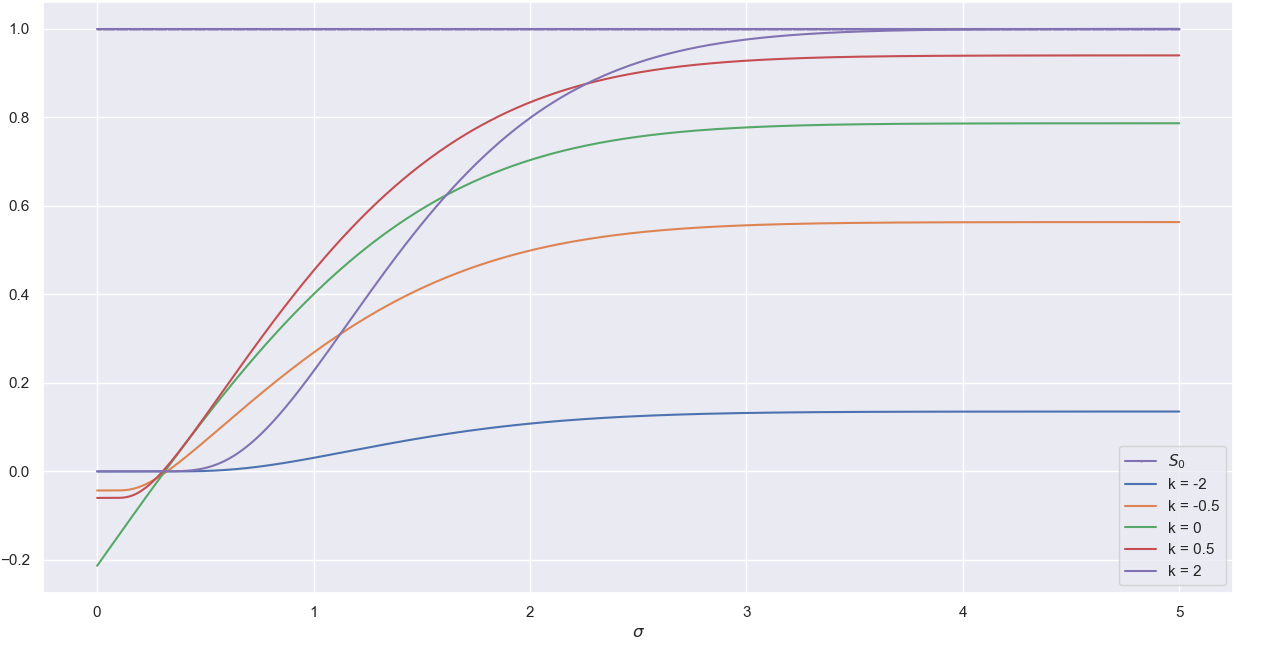
\includegraphics[width = 0.7 \textwidth]{../addition_part/images/annexe/vegaint.png}
\caption{Plot of the difference between the pricing for a call option between B$\&$S and under a Heston model, while varying $\sigma$ and the log strike price $k$.}
\label{fig:vegdif}
\end{figure}

\begin{figure}
\centering
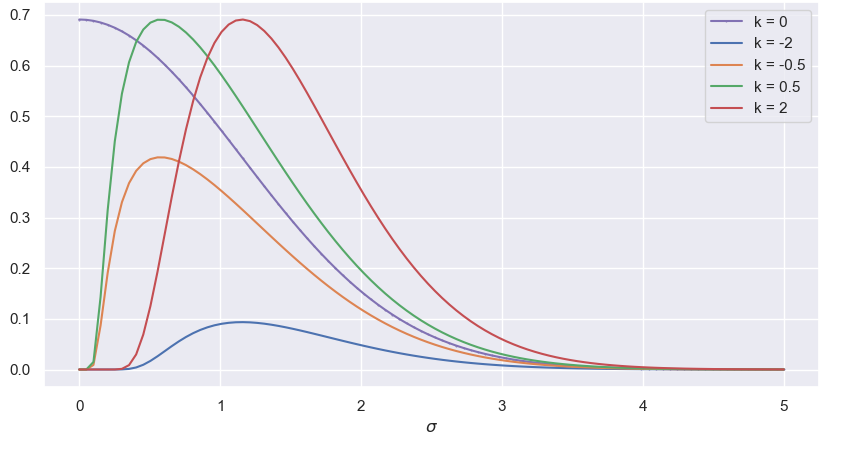
\includegraphics[width = 0.7  \textwidth]{../addition_part/images/annexe/vega.png}
\caption{Black and Scholes' vega varying with $\sigma$, under different log strike prices.}
\label{fig:vegabs}
\end{figure}










\section{Limiting cases}

\begin{figure}
\centering
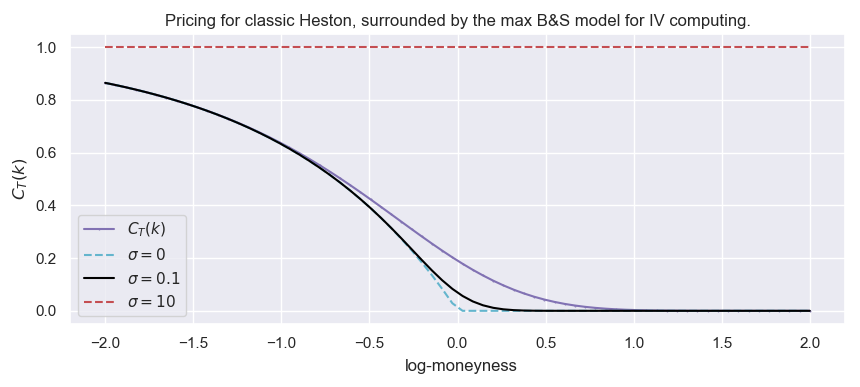
\includegraphics[width = \textwidth ]{../addition_part/images/annexe/pricing_IV.png}
\caption{Black and Scholes model for varying volatility.}
\label{fig:BSvolatilitymaxcase}
\end{figure}

The limiting cases for Black $\&$ Scholes for its volatility are the boundaries of our inversion range. The shape of the extreme cases are shown on fig. \ref{fig:BSvolatilitymaxcase}.

\begin{theoreme}{}
\begin{align}
\lim_{ \sigma \to 0^+} C_{T,K}^{BS} (\sigma) &= (S_0 - e^{-rT} K)^+ \\
\lim_{ \sigma \to +\infty } C_{T,K}^{BS} (\sigma) &= S_0  
\end{align} 
 
\end{theoreme}
\begin{remarque}
The philosophical meaning of that is that when there is no variance for the price, the best estimation of the mean is the function itself at the initial time. When the volatility goes to infinity, then nothing can be said about the option so it comes back to the price of the underlying asset.
\end{remarque}

In the following proof, one can either use as the argument $(*)$, the dominated convergence theorem, or this one :

\begin{theoreme}{Limit at infinity of composition of functions}
If a function $g:\mathbb R\to \mathbb R$ has a limit at $+\infty $, i.e. if there is $\ell\in\mathbb R\cup\{\pm \infty \}$ s.t. $$\lim_{x\to \infty }g(x)=\ell,$$
then $$\lim_{x\to \infty }g(h(x))=g\left(\lim_{x\to \infty }h(x)\right)=\ell,$$
whenever $h:\mathbb R\to \mathbb R$ is such that $$\lim_{x\to \infty }h(x)=\infty .$$ 
\end{theoreme}


\begin{demo}{}{}
What we want to compute is:
\begin{align*}
\lim_{ \sigma \to 0^+} C_{T,K}^{BS} (\sigma) 
&=  \lim_{ \sigma \to 0^+} \left ( S_0 \phi ( d_+ ) - e^{-r T } K  \phi( d_- ) \right ) \\
&= \lim_{ \sigma \to 0^+} \left ( S_0 \int_{- \infty}^{d_+} d (\phi) - e^{-r T } K  \int_{- \infty}^{d_+} d (\phi)  \right )\\
&=  (S_0 - e^{-r T } K )^+
\end{align*}
where one uses argument $(*)$ in the last line. It is obvious that since $\phi$ is a CDF, $\phi$ is bounded and the limit exists. 
Also :

\begin{align*}
\lim_{ \sigma \to 0^+} d_{+} &= \lim_{ \sigma \to 0^+} \frac{1}{\sigma \sqrt{T}  } \left ( \ln(\frac{S_0}{K}) + \left ( r + \frac{\sigma^2}{2} \right ) T \right ) \\
&= \text{sgn}(S_0 - K) \cdot \infty \\
\lim_{ \sigma \to 0^+} d_{-} &= \lim_{ \sigma \to 0^+} \frac{1}{\sigma \sqrt{T}  } \left ( \ln(\frac{S_0}{K}) + \left ( r - \frac{\sigma^2}{2} \right ) T \right ) \\
&= \text{sgn}(S_0 - K) \cdot \infty 
\end{align*}

the other limit is computed in a similar way.
\end{demo}


\chapter{Feller Condition}
\label{feller_condition}
\begin{theoreme}{Feller Condition}
When one assumes as a model the classical Heston model :
\begin{align}
d V_t &= \kappa  (  \phi - V_t ) dt + \sigma \sqrt{V_t} dB_t \\
d S_t &= S_t ( r_t + \theta V_t ) dt + S_t \sqrt{V_t} d W_{1,t} \\
d B_t &= \rho d W_{1,t} + \sqrt{1- \rho^2 } d W_{2,t} 
\end{align}

A suffisiant condition to have $V_t > 0$ is :
$$ 2 \kappa  \theta > \sigma^2 $$

\end{theoreme}
